% Where each implemented Runge--Kutta method samples f_theta inside one step, and with what
% weight. Nodes c_i and weights b_i are copied from implementation/ode/solvers.py
% (DOPRI5 and Tsit5: first six stages; the FSAL seventh stage has b_7 = 0 and is skipped).
\documentclass[tikz,border=4pt]{standalone}
\usepackage{amsmath,amssymb}
\usepackage{mathptmx}
\usepackage[scaled=0.90]{helvet}
\usetikzlibrary{arrows.meta,calc}

\definecolor{ink}{RGB}{28,32,38}
\definecolor{primary}{RGB}{155,26,32}
\definecolor{accentsoft}{RGB}{247,228,229}
\definecolor{rule}{RGB}{209,213,219}
\definecolor{blueacc}{RGB}{30,90,168}
\definecolor{muted}{RGB}{95,107,122}

% bar height per unit weight, and step width in cm
\def\bh{0.55}
\def\W{7.0}

\begin{document}
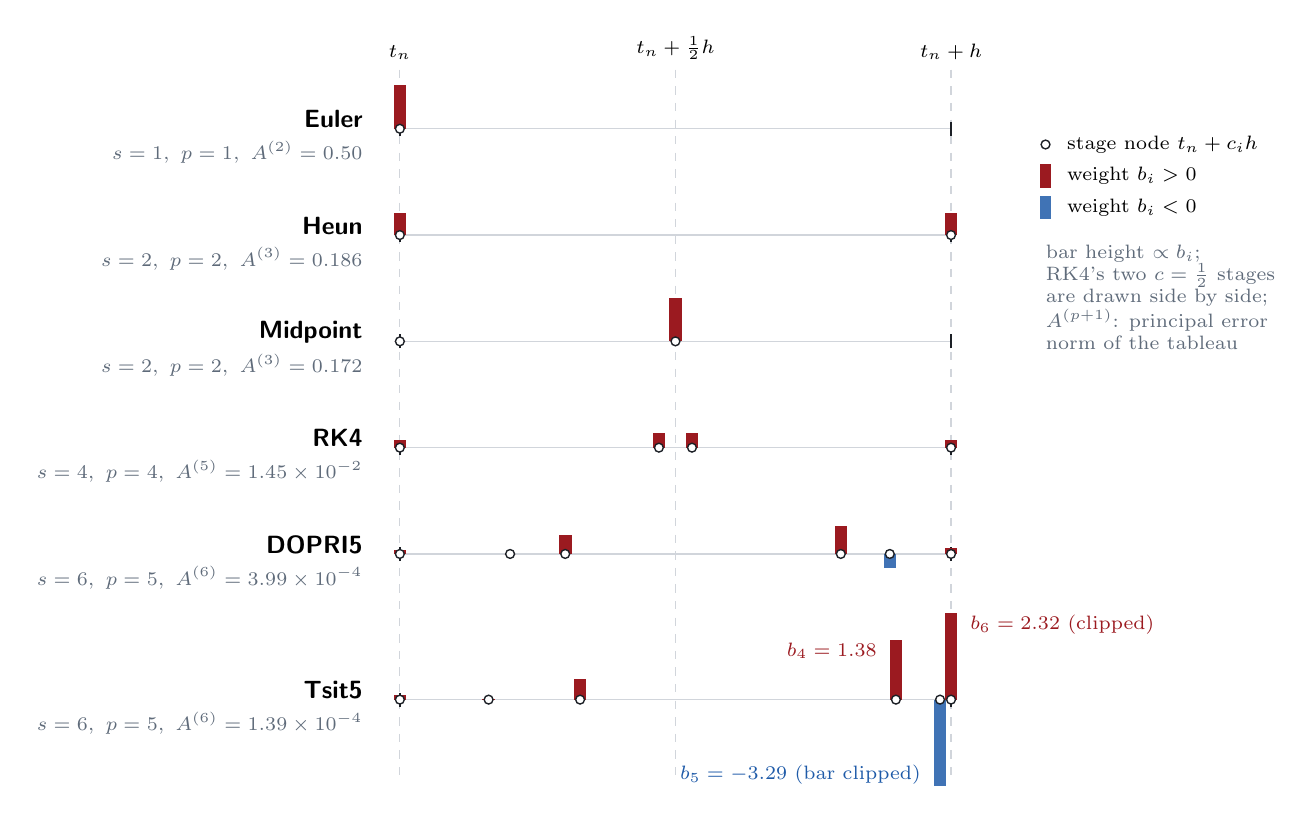
\begin{tikzpicture}[font=\sffamily\small]
\foreach \c in {0,0.5,1} \draw[rule, dashed, line width=0.4pt] ({\c*\W},0.75) -- ({\c*\W},-8.3);
% one row per method: name / stages / order / principal error norm / list of c:b pairs
\foreach \yy/\name/\meta/\pairs [count=\r] in {
  0/Euler/{$s=1,\ p=1,\ A^{(2)}=0.50$}/{0/1},
  -1.35/Heun/{$s=2,\ p=2,\ A^{(3)}=0.186$}/{0/0.5, 1/0.5},
  -2.7/Midpoint/{$s=2,\ p=2,\ A^{(3)}=0.172$}/{0/0, 0.5/1},
  -4.05/RK4/{$s=4,\ p=4,\ A^{(5)}=1.45\times10^{-2}$}/{0/0.16667, 0.47/0.33333, 0.53/0.33333, 1/0.16667},
  -5.4/DOPRI5/{$s=6,\ p=5,\ A^{(6)}=3.99\times10^{-4}$}/{0/0.09115, 0.2/0, 0.3/0.44923, 0.8/0.65104, 0.88889/-0.32237, 1/0.13095},
  -7.25/Tsit5/{$s=6,\ p=5,\ A^{(6)}=1.39\times10^{-4}$}/{0/0.09646, 0.161/0.01, 0.327/0.47989, 0.9/1.37901, 0.98003/-3.29007, 1/2.32471}%
} {
  \begin{scope}[yshift=\yy cm]
    \node[anchor=east, font=\sffamily\small\bfseries] at (-0.35,0.12) {\name};
    \node[anchor=east, font=\scriptsize\color{muted}] at (-0.35,-0.3) {\meta};
    \draw[rule, line width=0.5pt] (0,0) -- (\W,0);
    \draw[ink, line width=0.6pt] (0,-0.09) -- (0,0.09) (\W,-0.09) -- (\W,0.09);
    \foreach \c/\b in \pairs {
      \pgfmathsetmacro{\xx}{\c*\W}
      \pgfmathsetmacro{\hh}{max(-1.1,min(1.1,\b*\bh))}
      \pgfmathsetmacro{\neg}{\b<0 ? 1 : 0}
      \ifdim \neg pt > 0.5pt
        \fill[blueacc!85] (\xx-0.08,0) rectangle (\xx+0.08,\hh);
      \else
        \fill[primary] (\xx-0.08,0) rectangle (\xx+0.08,\hh);
      \fi
      \fill[white, draw=ink, line width=0.5pt] (\xx,0) circle (1.6pt);
    }
  \end{scope}
}
% clipped Tsit5 bar gets its true value printed
\node[font=\scriptsize, text=blueacc, anchor=east] at ({0.98003*\W-0.12}, {-7.25-0.95}) {$b_5=-3.29$ (bar clipped)};
\node[font=\scriptsize, text=primary, anchor=east] at ({0.9*\W-0.12}, {-7.25+0.62}) {$b_4=1.38$};
\node[font=\scriptsize, text=primary, anchor=west] at ({\W+0.12}, {-7.25+0.95}) {$b_6=2.32$ (clipped)};
% axis labels
\node[font=\scriptsize, anchor=south] at (0,0.75) {$t_n$};
\node[font=\scriptsize, anchor=south] at (\W,0.75) {$t_n+h$};
\node[font=\scriptsize, anchor=south] at ({0.5*\W},0.75) {$t_n+\tfrac12 h$};
% legend
\begin{scope}[shift={(\W+1.2,-0.2)}]
  \fill[white, draw=ink, line width=0.5pt] (0,0) circle (1.6pt);
  \node[anchor=west, font=\scriptsize] at (0.15,0) {stage node $t_n+c_i h$};
  \fill[primary] (-0.07,-0.55) rectangle (0.07,-0.25);
  \node[anchor=west, font=\scriptsize] at (0.15,-0.4) {weight $b_i>0$};
  \fill[blueacc!85] (-0.07,-0.95) rectangle (0.07,-0.65);
  \node[anchor=west, font=\scriptsize] at (0.15,-0.8) {weight $b_i<0$};
  \node[anchor=north west, font=\scriptsize, align=left, text=muted] at (-0.12,-1.15)
    {bar height $\propto b_i$;\\RK4's two $c=\tfrac12$ stages\\are drawn side by side;\\$A^{(p+1)}$: principal error\\norm of the tableau};
\end{scope}
\end{tikzpicture}
\end{document}
